\chapter{TLDR Design and Implementation}
\label{sec:Implementation}

In this section, we discuss the design and implementation of TLDR. We first discuss the main algorithms of TLDR, and show how they can be parallelized. Then we describe the architecture of the implementation and each module in detail. 

\section{Test Selection and Dependency Extraction}

Algorithm \ref{tldr} describes the test selection algorithm underlying TLDR. The procedure takes two versions of a project as input -- $project_{n}$ and $project_{n-1}$ -- and returns the set of selected tests, $selected$. It does so by iterating through all class files of the latest version, checking for new, modified, and deleted ones. For new and modified classes, it then iterates through their declared members (methods and fields), checking for new, modified, and deleted members. For new and modified members, it extracts their static dependencies -- an algorithm explained next. Changes in classes and members are calculated by the checksum of their corresponding byte code using \textit{BLAKE2B}~\cite{aumasson2013blake2}, an efficient checksum algorithm. 

After updating the dependency graph, algorithm \ref{tldr} then generates $goldset$, which is a set of all members that may have indirectly been affected by changes in $project_{n-1}$, by performing a depth-first search (DFS) over the dependency graph (line 30 of the algorithm). Each method or field in $goldset$ is mapped to one or more tests that have dependencies on those entities. Test methods may have dependencies on other test methods and fields. Therefore, in order to select all impacted tests, transitive dependents of each test method in $mapped$ are collected. Finally, the set of tests, $selected$, is generated by another DFS in the dependency graph, but this time only traversing test-test dependency edges. 

\begin{algorithm}
{\fontsize{12pt}{12pt}\selectfont
\caption{Test Selection pseudo-code}
  \label{tldr}
  \begin{algorithmic}[1]
\Function{TLDR}{$project_{n}, project_{n-1}$}
\State $new, changed, goldset, mapped, selected \Leftarrow \phi$

\ForAll{\colorbox{blue!30}{$file_{n} \in project_{n}$}}
    \If{$file_{n} \notin project_{n-1}$}
        \State $\textit{insert}(file_{n}, \textit{blk2b}(file_{n}))$
    \EndIf
    \If{$\textit{blk2b}(file_{n})\neq\textit{blk2b}(file_{n-1})$} 
      \State $\textit{update}(file_{n}, \textit{blk2b}(file_{n}))$
      \ForAll{\colorbox{blue!30}{$member_{n} \in file_{n}$}}
           \State $extract = false$
          \If{$member_{n} \notin project_{n-1}$}
                \State $\textit{insert}(member_{n},  \textit{blk2b}(member_{n}))$
                \State $new = new \cup \{member_{n}\}$ 
                \State $extract = true$
          \ElsIf{$\textit{blk2b}(member_{n})\neq\textit{blk2b}(member_{n-1})$}
                 \State $\textit{update}(member_{n}, \textit{blk2b}(member_{n}))$
                 \State $changed = changed \cup \{member_{n}\}$ 
                 \State $extract = true$
          \EndIf
          \If{$extract\land isMethod(member_n)$ } 
                    \State $DEPEXTRACTION(member_{n})$
          \EndIf
          
          \ForAll{$member_{n-1} \in project_{n-1} - project_{n}$}
               \State $remove(member_{n-1})$
            \EndFor    
            
       \EndFor
    \EndIf
\EndFor

\ForAll{\colorbox{blue!30}{$member \in new \cup changed$}}
        \State $goldset = goldset \cup \textit{dfs(member)}$ 
\EndFor

\ForAll{\colorbox{blue!30}{$member \in goldset$}}
        \State $mapped = mapped \cup \textit{testmap(member)}$ 
\EndFor

\ForAll{\colorbox{blue!30}{$test \in mapped$}}
        \State $selected = selected \cup \textit{dfs(test)}$ 
\EndFor\\
\Return ${selected}$
\EndFunction
\end{algorithmic}
}
\end{algorithm}



\begin{algorithm}
{\fontsize{12pt}{12pt}\selectfont

\caption{Dependency Extraction pseudo-code}
  \label{dependency}
  \begin{algorithmic}[1]

\Function{DEPEXTRACTION}{$entity$}

\State $direct \Leftarrow $\{ $"putstatic"$, $"putfield"$, $"getstatic"$, $"getfield"$\}
\State $polymorphic \Leftarrow $\{$"invokevirtual"$, $"invokeinterface"$, $"invokestatic"$, $"invokespecial"$\}
\State $dependencies \Leftarrow \phi$\\

\LineComment[1\dimexpr\algorithmicindent]{Extract dependencies from method bytecode}
\ForAll{$instruction \in entity.bytecode$}
     \If{$instruction.type \in (direct \cup polymorphic) $}
         \State $dependencies = dependencies \cup instruction.callee$ 
     \EndIf
\EndFor
\ForAll{$member \in dependencies$}
    \If{$\textit{dep\_type(entity, member)} \in direct$}
        \State $ \textit{insert\_in\_db(entity, member)}$
    \ElsIf{$\textit{dep\_type(entity, member)} \in polymorphic$}
        \State $hierarchy \Leftarrow classHierarchy(member)$
        \If{$isOverridden(member, hierarchy)$}
            \State $nodes \Leftarrow getOverrides(member, hierarchy)$ 
        \ElsIf{$isMissing(member, class(member))$}
            \State $nodes \Leftarrow getInherited(member, hierarchy)$ 
        \EndIf
        \ForAll{$e \in nodes$}
        \State $ \textit{insert\_in\_db(entity, e)}$
        \EndFor
    \EndIf
\EndFor

\EndFunction
\end{algorithmic}
}
\end{algorithm}
\medskip

For each changed or new $file$, Algorithm~\ref{tldr} finds all new and changed members, and updates the dependency graph of changed methods by calling Algorithm~\ref{dependency}, our dependency extraction algorithm. This algorithm takes a method that has been changed and updates the global dependency graph by processing the bytecode of that method looking for instructions that establish dependencies to other methods and fields. Those dependencies may be direct (e.g. {\em putfield} establishes a dependency to the immediate target of the invocation) or indirect, which may involve polymorphic relations (e.g. {\em invokevirtual} involves dynamic dispatch, meaning that the exact type of the target is only known at runtime). Since JVM specification allows static methods to be polymorphic as well, we consider  {\em invokestatic} as polymorphic method invocation as well. In the case of a polymorphic target, we conservatively traverse the class hierarchy of that target either up or down, in search of all possible polymorphisms. For example, when the target is a method that is overridden in one or more subclasses of its class, we include all those overridden methods as dependencies, because we don't know the exact method that will be called at runtime; similarly, when the target is missing the method, it means that the method is inherited from a superclass. In this case, we have to traverse up in the class hierarchy and include the superclass method as a dependency.

\section{Safety}
An RTS technique is {\em safe} iff it selects all tests that are impacted by a change in the projects' files~\cite{willmor2005safe}. As currently implemented, TLDR is not entirely safe, because it does not track dependencies resulting from (a) the use of Java reflection, and (b) the use of external jars. This is not an inherent problem of TLDR; it is simply a limitation of its current implementation, which we plan to improve. This limitation affects other RTS tools that are based on static analysis~\cite{starts, hyrts, rtsplusplus}. TLDR is safe for all other cases, i.e. for {\em all} changes in the {\em source files} of the projects, as long as they don't involve reflection. 
In broad strokes, an RTS technique is safe when (1) it correctly captures all dependencies of all code entities down to the desired level of granularity; (2) it correctly slices the dependency graph for the set of entities that change from a version to another; and (3) it correctly identifies the tests that reach any part of those slices. For performance purposes, and as explained above, TLDR uses a static dependency graph. Because of dynamic dispatch, static analysis of object-oriented programs needs to take inheritance relations into account. Algorithm~\ref{dependency} describes the construction of this static extended dependency graph, which is complete, with the two exceptions: reflection and external jars. While constructing the static extended call dependency graph, it considers both direct (line (12)) and polymorphic (line (14)) dependencies.  

\section{Parallelism in TLDR}

The algorithms described above are not particularly new -- similar techniques for change analysis were used by other RTS tools~\cite{faulttracer, hyrts, ekstazi, starts}. However, in TLDR, we leverage the potential that Algorithm~\ref{tldr} has for parallelism to reduce test selection overhead. Specifically, instead of sequentially executing the entire algorithm, we parallelize lines (3), (9), (29), (32), and (35) -- these are portions of the algorithm that map certain processing functions to potentially large numbers of classes and their members.

\begin{figure*}
\begin{center}
  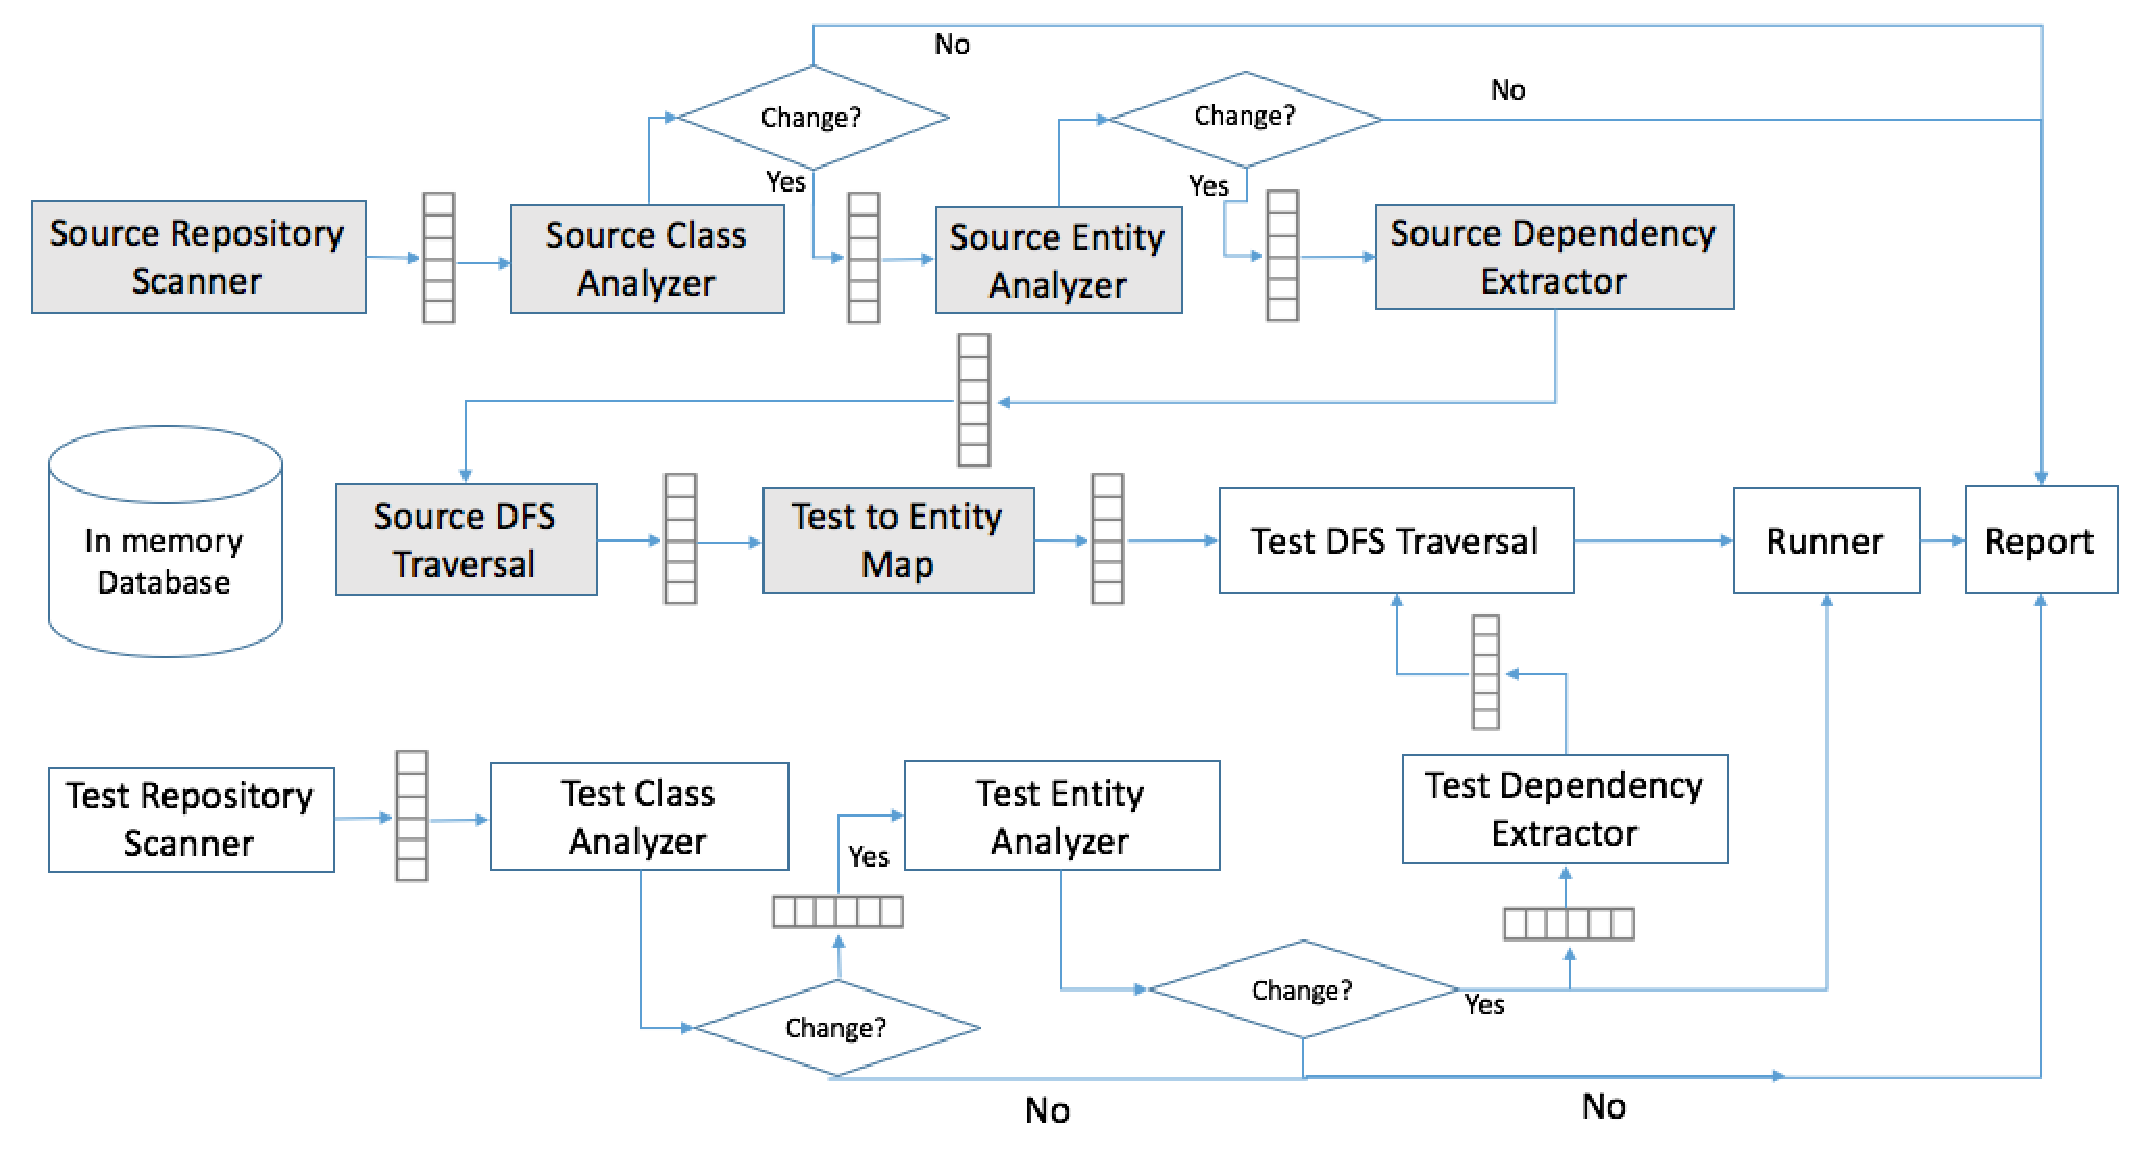
\includegraphics[width=18cm,height=8.5cm]{arch}
  \caption{Pipe-and-filter architecture of TLDR. The architecture contains two partially-independent pipelines, one for the source-code (marked as grey) and one for the test-code (marked as white).}
  \label{fig:tldr}
\end{center}
%\vspace{-5ex}
\end{figure*}

Figure \ref{fig:tldr} depicts the pipe-and-filter architecture of TLDR, which fully leverages parallelism for test selection and implements Algorithm~\ref{tldr}. The data elements of the pipeline are the absolute paths of the class files -- and the fully qualified name of the classes, methods, and fields. The pipeline takes as input the absolute path of each class file and outputs a set of selected tests. Components in the pipeline are multi-threaded and interact with each other through queues. The number of worker threads between two components is configurable, so to better take advantage of the hardware. As a result, TLDR can use the full computational power of each machine where it runs. 

TLDR's architecture contains two sub-pipelines: one associated with the source code under test -- which we refer to as the \textit{source pipeline} and whose constituent components are colored in grey -- and another associated with test code of the project -- which we refer to as the \textit{test pipeline} and whose constituent components are filled in white. These two pipelines operate in parallel and either asynchronously or synchronously, depending on which component is currently operating. Broadly, each of these two sub-pipelines has the following four components in common: \textit{Repository Scanner, Class File Analyzer, Entity Analyzer, Dependency Extractor}. Ultimately, these two sub-pipelines merge in the \textit{Test DFS Traversal} component, followed by execution of tests by the \textit{Runner} module. In the remainder of this section, we describe the functionality of each component.  

\section{In-Memory Database}
Deductive databases are often used to store program information as relations for numerous program analyses~\cite{lam2005context}. Similar to other RTS tools, we store program-specific information for incremental change analysis, dependency graph traversals, and mapping entities to a test method~\cite{faulttracer, hyrts, starts, ekstazi, legunsen2016extensive}. 

Data storage and retrieval are expensive processes. If nothing changes in the project, TLDR at a minimum needs to retrieve previously stored checksums of each class file for \textit{change impact analysis}, i.e. determining the entities affected by a change to another entity. Therefore, performance of RTS greatly depends on the database schema as well as storage technology.  To achieve high performance, we use an in-memory database server, \textit{Redis}. We implemented a customized \textit{database handler} which is available to all the components in the pipeline. The database handler provides thread-safe APIs to read, update, and delete values.

\begin{table}
  \scriptsize
  \centering
  \caption{Hashtables used by TLDR's In-Memory Database}
    \begin{tabular}{r | ll}
    \multicolumn{1}{l|}{\textbf{Hashtable No.}}  & \textbf{Key} & \textbf{Value} \\
    \hline
    1     & class absolute path & checksum \\
    2     & FQN of entity & checksum \\
    3     & FQN of entity & set of FQN of dependent entity \\
    4     & FQN of entity & set of FQN of dependency entity \\
    5     & FQN of Class & set of FQN of super class and interfaces \\
    6     & FQN of Class & set of FQN of the subclasses \\
    7     & FQN of entity & set FQN of test methods \\
    8     & FQN of test entity & Boolean \\
    \hline
    \end{tabular}%
  \label{tab:hashtables}%
\end{table}


\vspace*{0.2cm}
\noindent

Conceptually, Redis tables are hashtables, i.e. key-value pairs. In TLDR, the keys are the fully qualified name (FQN) of the entities and the values are either a hashcode, i.e. checksum, or a set of FQNs. Table \ref{tab:hashtables} shows the 8 hashtables used by TLDR, each identified with a table ID. Hashtable 1 and 2 store the checksum of each file and entity i.e. field and method respectively. These two hashtables used for change analysis. Hashtable 3 stores the set of dependents of each field and method. This table is the dependency graph of the project. It is used by the DFS algorithm to traverse the firewall of each changed field and method. Hashtable 4 is the inverse of hashtable 3. It stores the set of dependencies of each field and method. This table is needed for faster update of hashtable 3 when a method is no longer another method's or a field's dependent. Hashtable 5 stores class-hierarchy information. This table is used by algorithm \ref{dependency} to construct polymorphic edges in the dependency graph. Hashtable 6 is the inverse of hashtable 5 and facilitates faster update of hashtable 5 when the class hierarchy of the projects changes. Hashtable 7 stores entity to test mapping information. This is used in mapping tests to each field and method in $goldset$ in algorithm \ref{tldr}. Hashtable 8, stores all test methods and fields. This table is used along with table 3 to traverse within the test suite. 


\section{Repository Scanner}

\noindent
Both the source and test pipelines start by scanning the repository of the project using a recursive depth-first search algorithm that locates all class files in the repository. In a Maven project, source classes reside on \textit{*/target/classes/} directory and test classes reside on \textit{*/target/test-classes/} directory. Source Repository Scanner collects all source classes and Test Repository Scanner collects all test classes from the above-mentioned directories respectively. A Maven project can be hierarchical with multiple modules. Each module can have its own independent source and test directory. Each Repository Scanner can discover all such source and test directories. 

\section{ Class Analyzer and Entity Analyzer}

TLDR performs change impact analysis during two subsequent stages: one for the class level and another for the method- and field-level. TLDR analyzes change at the bytecode level. We choose this level because many changes that do not affect tests can be filtered out when analyzing bytecode but would result in unnecessary test selection at the source code level. For instance, new or changed comments or equivalent code at the statement level (e.g., \textit{var++} instead of \textit{var = var + 1}), etc. yields the same checksum. Previous testing approaches have followed a similar practice~\cite{ekstazi, hyrts, starts, xu2007regression, fraser2011evosuite}. 

Broadly, TLDR can detect 16 types of changes, shown in Table \ref{tab:changes}. Altogether, these 16 change types cover a wide variety of possible changes in object-oriented languages and at least the same type of changes handled by state-of-the-art RTS techniques \cite{ekstazi, hyrts, starts}.

\begin{table}
  \scriptsize
  \centering
  \caption{Changes detected by TLDR}
    \begin{tabular}{r | ll}
    \multicolumn{1}{l|}{\textbf{}}  & \textbf{Type of Change} \\
    \hline
    1     & Addition of a new class \\
    2     & Addition of a new method \\
    3     & Addition of a new field \\
    4     & Addition of a new static initializer \\
    5     & Change of a method definition \\
    6     & Change of a field value\\
    7     & Change of the class hierarchy \\
    8     & Change of a class signature \\
    9     & Change of a field signature \\ 
    10    & Change of a method signature \\ 
    11    & Change of a static initializer \\ 
    12    & Deletion of a class \\ 
    13    & Deletion of a method \\ 
    14    & Deletion of a field \\ 
    15    & Deletion of a test case \\
    16    & Deletion of a static initializer \\
    \hline
    \end{tabular}%
  \label{tab:changes}%
\end{table}%

TLDR uses a 16 character-long alpha-numeric checksum as part of its change impact analysis. The efficiency of the test selection pipelines also depends on checksum calculation. To maximize efficiency of checksum usage, TLDR uses \textit{BLAKE2B}~\cite{aumasson2013blake2}, which is 4 to 8 times faster than \textit{SHA256, BLAKE, and SHA-1}. 

For each \textit{Class File Analyzer}, i.e., source and test, TLDR calculates the checksum of bytecode. Only the class files whose checksums are different than the previously computed value are forwarded to the next component in the pipeline for field- and method-level change analysis as shown in figure\ref{fig:change_class}. 

\begin{figure*}
\begin{center}
  \includegraphics[width=14cm,height=6.5cm]{redis}
  \caption{Change analysis of class files. Only the changed class files are passed to the next module.}
  \label{fig:change_class}
\end{center}
\end{figure*}

For both source and test \textit{Entity Analyzer} components, TLDR splits the class file into methods and fields using \textit{Apache Common BCEL} library. The checksum is calculated by concatenating the entity's (i.e., method's or field's) modifier, signature, and body. We omit \textit{StackMap Table} of the methods. The offset delta of StackMap of a method depends on the overall offset of the class file. Addition or deletion of a statement in the preceding method can possibly change the offset information of the subsequent methods' StackMap Table. This can cause changes in the checksum of a method even though that method did not change in code. 


\begin{figure*}
\begin{center}
  \includegraphics[width=16cm,height=7.5cm]{class}
  \caption{Change analysis of methods and fields. Each changed class file is split into methods and fields and fed to the change analysis module.}
  \label{fig:change_method}
\end{center}
\end{figure*}


For fields, we calculate the checksum of the signature of the field. In addition to change analysis, we perform three tasks in Entity Analyzer: (1) extracting the class-hierarchy information, i.e., super-class and interfaces of the class; (2) update the class-hierarchy information in the database if the class hierarchy is changed; (3) update and sync the dependency information if a method or field has been deleted. 

\section{ Dependency Extractor}

\noindent
Algorithm \ref{dependency} implements Dependency Extractor. For each method including constructors (\texttt{<init>}) and static initializer (\texttt{<clinit>}), both source and test, we extract dependencies by parsing the operands of the following 13 bytecode instructions: i) \texttt{invokestatic}, ii) \texttt{invokespecial}, iii) \texttt{invokevirtual}, iv) \texttt{invokeinterface}, v) \texttt{getstatic}, vi) \texttt{getfield}, vii) \texttt{putstatic}, viii) \texttt{putfield}, ix) \texttt{checkcast}. For \texttt{invokevirtual}, \texttt{invokeinterface}, \texttt{invokestatic}, and \texttt{invokespecial} we retrieve all overridden versions of the dependency method by traversing the class hierarchy. 

The extracted dependency information is inserted in both a forward and inverted index of dependencies. The inverted index is being used to formulate the transitive dependents of the changed methods, while the forward index is being used to update and synchronize the database in case a dependency is deleted in a particular revision. For the test pipeline, dependency information is indexed into two tables: (1) Hashtable 3 and (2) Hashtable 7. Test dependencies on source methods are used to map a source entity to a test method. Test methods have dependencies to other test members. To select all impacted test methods, we have to find the transitive dependents of each test that mapped to a method or field in $goldset$. 

%Test dependencies to other test methods are used to traverse the transitive dependencies among test methods. Data from this module is forwarded to the DFS Traversal Component for subsequent analysis. 

\vspace*{0.2cm}
\noindent
\subsection{ DFS Component}

\noindent
This component is a Depth-first search algorithm that traverses the transitive dependency of each changed or newly added entity. DFS Traversal of the source pipeline is synchronized with the Dependency Extractor of the test pipeline. Algorithm \ref{tldr} waits for Test Dependency Extractor to finish for all data elements in the test pipeline before forwarding each member in $goldset$ to Test to Entity Map component. This is because in order to map the source members to test methods, all test methods must be parsed and their updated dependency to the source methods must be indexed. Source DFS Component collects the firewall of each changed or new member. 

The DFS component of the test pipeline gets input from both Test Dependency Extractor of the test pipeline and Test to Entity Map component of the source pipeline. This module is the meeting point of the two sub-pipelines. Test methods might have dependencies on other test fields, parameterized test methods, or helper methods. Test DFS component allows traversing these transitive dependencies for each new or mapped test method. This component is customized to traverse transitive dependency within the test suite.


\section{Test to Entity Map}

This component is only present in the source pipeline. This is a mapping function that maps each entity in the transitive dependent set of each changed or newly added method and field to a test method, i.e., a test method which has a direct dependency on one or more entities in the transitive dependent set. Mapped tests are then forwarded to test DFS Traversal to form a transitive set of impacted changed methods. 

\section{Runner}

TLDR extends \texttt{Maven SureFire} which is a plugin to run JUnit tests in Maven projects. TLDR runs the only the selected tests by dynamically updating the \texttt{test} field of \texttt{SureFire} by Java instrumentation. In order to run the selected tests parallelly, TLDR updates \texttt{SureFire} configuration values -- \texttt{forkCount} and \texttt{reuseForks}. These flags enable Surefire to spawn a specified number of JVM processes and distribute test run load among the processes parallelly.


\section{TLDR Artifact}

TLDR is an open-source project. TLDR's source-code can be found in this GitHub repository : \href{url}{http://www.github.com/Mondego/TLDR}. The tool has not been released in the Maven Central Repository yet. Therefore, it needs to be installed in the local maven repository. To do so, the source-code needs to be cloned into the local machine and within the repository, the following maven command is needed to be executed \textit{mvn clean compile install}. After installing TLDR in the local maven repository, the following XML snippet needs to be added in the \textit{<plugins>} block of the \textit{pom.xml} file of the project which is to be tested through TLDR. 
\newline
\begin{lstlisting}
<plugin>
	<groupId> com.mondego.ics.uci </groupId>
	<artifactId> tldr-plugin </artifactId>
	<version> 1.0.2-SNAPSHOT </version>
	<configuration>
		<goalPrefix> tldr </goalPrefix>
		<skipErrorNoDescriptorsFound> true </skipErrorNoDescriptorsFound>
	</configuration>				
</plugin>
\end{lstlisting}

Before running the plugin, a Redis server must be started locally. Finally, the following command should be executed - 
\textit{mvn com.mondego.ics.uci:tldr-plugin:1.0.2-SNAPSHOT:tldr -Dmultimodule.projectname=<project-name>}. This will invoke Maven surefire and the test report will be placed inside the \textit{Target} folder of the repository. TLDR provides several optional command-line options. Some relevant command-line options are as follows -

\begin{itemize}
    \item -Ddebug.flag: turns on the debug prints during different stages of the pipeline. 
    \item -Dlog.directory: specifies the location of log files that are generated during analysis and testing.  
    \item -Dcommit.hash: specifies the hashcode of a particular commit on which TLDR is to be run.
    \item -Dcommit.serial: specifies the serial number of the project iteration. This flag is useful in iterative evaluation of TLDR.
    \item -Dfork.count: specifies the number of process forks test runner should use. 
    \item -Dthread.count: specifies the number of threads the test runner should use. 
 \end{itemize}
